\documentclass[12pt,oneside,a4paper,english]{article}
\usepackage[T1]{fontenc}
\usepackage[latin2]{inputenc}
\usepackage[margin=2.25cm,headheight=26pt,includeheadfoot]{geometry}

\usepackage{listings}
\usepackage{color}
\usepackage{titlesec}
\usepackage{titling}
\usepackage[framed, numbered]{matlab-prettifier}
\usepackage{changepage}
\usepackage{amsmath}
\usepackage{hyperref}
\usepackage{enumitem}
\usepackage{graphicx}
\usepackage{fancyhdr}
\usepackage{lastpage}
\usepackage{caption}
\usepackage{tocloft}
\usepackage{setspace}
\usepackage{multirow}
\usepackage{titling}
\usepackage{float}
\usepackage{comment}
\usepackage{booktabs}
\usepackage{indentfirst}
\usepackage{lscape}
\usepackage[english]{babel}
\usepackage{booktabs,caption}
\usepackage[flushleft]{threeparttable}
\usepackage[english]{nomencl}
\usepackage{xcolor}
\usepackage{lipsum}

% --- set footer and header ---
\pagestyle{fancy}
\fancyhf{}

\setlength{\parindent}{2em}
\title{Thesis} % to reference as \title, dont use \maketitle
\makeatletter\let\Title\@title\makeatother

\lstset{language=Matlab,
style=Matlab-editor,
basicstyle=\normalsize\mlttfamily,
numbers=left,
numberstyle={\scriptsize\color{black}},			% size of the numbers
numbersep=0.5cm											
}

\newlist{steps}{enumerate}{1}
\setlist[steps, 1]{leftmargin=1.5cm,label = Step \arabic*:}
\renewcommand{\headrulewidth}{1pt}
\renewcommand{\footrulewidth}{1pt}

%\lhead{\Title}
\rhead{\nouppercase{\rightmark}}
\lhead{\Title}
%\rfoot{
\includegraphics[height=1.25cm]{root/logo.pdf}} % right header logo
\setlength\headheight{16pt}
\setlength{\footskip}{50pt}
\lhead{\Title} %rightH title
\cfoot{\thepage}

% --- End of page settings ---



\begin{document}
\pagenumbering{roman} 

\begin{titlepage}
\begin{center}
\vspace{2cm}

% Title

\vspace{2.5cm}
{ \huge \bfseries Technical University of Crete} % title of the report
\vspace{2.5cm}


%\textsc{ Danmarks Tekniske Universitet}\\[1.5cm]

\includegraphics[width=0.2\textwidth]{root/tuc.png}~\\[1cm]
\vspace{2cm}

\vspace{2cm}

% Title
\hrule
\vspace{.5cm}
{ \huge \bfseries Title\\ of the Thesis} % title of the report
\vspace{.5cm}

\hrule
\vspace{1.5cm}

\textsc{\textbf{Authors}}\\
\vspace{.5cm}
\centering

% add your name here
Kyriakos Christodoulidis\\

\vspace{4cm}

\centering \today 

\vspace{4cm}

\textsc{\textbf{Thesis Committee}}\\

\vspace{1cm}

Professor Mania Aikaterini (Supervisor)\\
Professor Chalkiadakis Georgios\\
Professor Michail G. Lagoudakis\\
\end{center}
\end{titlepage}

\newpage
\doublespacing
%\addcontentsline{toc}{section}{Abstract}
%\addcontentsline{toc}{section}{Acknowledgments}
\renewcommand{\baselinestretch}{1}\normalsize
\tableofcontents
\renewcommand{\baselinestretch}{1}\normalsize
\singlespacing
\thispagestyle{fancy} % force page style
\newpage
\pagenumbering{arabic} 
\fancyfoot[C]{Page \thepage\ of \pageref{EndOfText}}
\newpage
\addtocounter{section}{-1}
\section{Abstract}
\addtocounter{section}{-1}
\newpage
\section{Acknowledgments}
\newpage
\section*{Chapter 1 \\}
\section{Introduction}
\subsection{The increased demand of mocap clips}
Motion Capture (MoCap) is a cutting-edge method of capturing all or part of an actor's performance so that it can be translated into the action of a computer generated 3D character on screen. More specifically, the exact movements of the actor are captured and rendered onto the digital character. 

In the last years, there is a growing demand for MoCap in many fields including interactive virtual reality, film production, animation and so forth \cite{Efficient Content-Based Retrieval of Motion Capture Data}. However, capturing motions when needed is often not practical as motion capture systems are expensive and the capture processes are complex in general. It is often desirable to retrieve and reuse motion clips that have been captured before and stored in databases. Straightforwardly, the retrieval may be done based on text labels of motion clips. 

Therefore, using MoCap clips for production consists of the following problems. Firstly, there are a limited amount of MoCap clips that can be used and using something more unique means that the production must have the budget and the time to support it. Secondly, the majority of the stored databases of MoCap are not free to use or have poor quality.
 
\subsection{Thesis aim}
A new approach to resolving these issues is to address the problem with Neural Networks. More specifically, in this thesis, we propose a composition of a deep neural network \cite{Exploiting temporal information for 3D pose estimation} that will estimate the 3D human pose, and the output of the DNN will be saved into a Bio-vision Hierarchy (BVH) file. The task is to predict a pose skeleton for the person in each image of a video. Currently, human pose estimation is one of the challenging fields of study in computer vision which aims in determining the position or spatial location of body keypoints (parts/joints) of a person from a given image or video. 

The first step is to use a pre-trained deep neural network that can estimate these 2D keypoints. Afterward, \cite{3D Human Pose Estimation from Deep Multi-View 2D Pose,3D Human Pose Estimation Using Convolutional Neural Networks with 2D Pose Information} in order to achieve our goal we will use another pretrain model that will be fed with a 2D pose estimation as the input, estimates the 3D pose. However, estimating a 3D human pose from a single image is more challenging than 2D cases due to the lack of depth information, so the accuracy drops significantly. In order to increase the quality of the estimation, we suggest using the butter-worth filter, which removes noise from data without affecting the motion. After obtaining the smoothed 3D human pose, we need to create a skeleton, based on the joints that the first model estimated and import the keypoints to each corresponding bone. Finally, the BVH file will be created and it can be further cleaned manually by an animator in any 3D computer graphics software (Blender, Maya, AutoDesk). 

However, the code implementation will be in python, and most animators may struggle to install and run the code. In order to avoid this issue, we developed a Windows Application, that anyone can use that runs the python code of the Thesis.  
\subsection{Thesis Structure}
This thesis is organized in 6 Chapters:

	\begin{itemize}
		\item Chapter 1\\\\
            In this Chapter we discuss about the problems of the MoCap clips production and propose a solution to it. 
		\item Chapter 2\\\\
            In this Chapter, we provide the reader with a overview of some knowledge about MoCap Clips, as well as some pioneer studies and state the novelties of this study. Then, we present an approach with Generative Adversarial Networks (GAN's) that was a possible solution of the problematic situation, and the reasons that we aborted this solution.
		\item Chapter 3\\\\
		    In this Chapter, we show the reader the minimum requirements of the hardware that the proposed DNN needs in order to run. In addition, we suggest to the users the best case scenarios of the input, in order to improve the algorithm estimation. Finally, we present the Interface of the Windows Application UI.  
		\item Chapter 4\\\\
            In this Chapter, we explain the implementation of the algorithm as well as some important knowledge that is covered in the thesis. More specifically, the reader will be introduced to some pretrained models that are essential to the solution, and the procedure that these models use in order to estimate the orientation and location of the person. Having created the BVH file, we develop an Animator Tool, that animators can use to improve the results. Finally, we present the python library that allows us to convert the python code to a Windows Application, as well as the features of the Application. 
		\item Chapter 5\\\\
            In this Chapter, we compare the performance of the pretrained models in the ideal circumstances for each model. Moreover, we calculate the accuracy between a real and generated clip, and the reader will learn the circumstances that our model needs in order to work at its best.
		\item Chapter 6\\\\
            In this Chapter, we summarize our results and discuss our contribution. Finally, we address the disadvantages of our approach as well as some future ideas that would improve our work. 

	\end{itemize} 

\newpage
\section*{Chapter 2 \\}
\section{Background}
\subsection{Mocap clips}
Many different disciplines use motion analysis systems to capture human body movement and posture. Basic scientists want to learn more about the mechanisms that are used to translate muscular contractions about articulating joints into functional accomplishments like walking. Researchers are increasingly attempting to better understand the relationship between the human motor control system and gait dynamics.

Motion capture \cite{Review on Motion Capture Technology} is now widely used in the gaming, film, and animation industries to provide quick, low-cost body and/or facial animations in order to animate one or more characters. Animation processes did not see significant innovation until computers were introduced into the process. With the invention of key-framing, which reduced the number of samples required to create an animation, animators' jobs became much easier. This was a time-consuming process because, at the time, each artist was required to individually animate each pose/frame. With the introduction of key-framing, the artist specified the beginning and ending frames of the animation, while the intermediate frames of the movement were generated automatically. Some animations, however, remained impossible to recreate due to their inherent complexity, such as the human walking animation, which is too complex due to our articulations.

\begin{figure}[h]
	\centering
	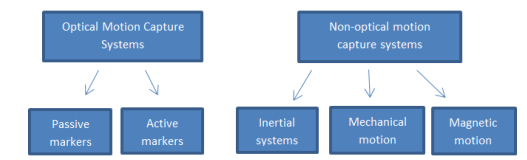
\includegraphics[width=0.7\textwidth]{figures/Mocap.png}
	\caption{MoCap systems Hierarchy}
\end{figure}

Motion analysis data collection protocols, measurement precision, and data reduction models have all been developed to meet the needs of their respective settings. Sport assessments, for example, necessitate higher data acquisition rates due to higher velocities than normal walking. Furthermore, real-time tracking is required for a realistic user experience, so time lag should be kept to a minimum. Years of technological advancement have resulted in numerous systems that can be classified as optical and non-optical, where non-optical category contains mechanical, magnetic, or inertial trackers. The human body is frequently viewed as a network of rigid links connected by joints. Human body parts are not rigid structures, but they are commonly treated as such during human motion studies. 
\pagebreak
\subsubsection{Optical Motion Capture}

\begin{figure}[h]
	\centering
	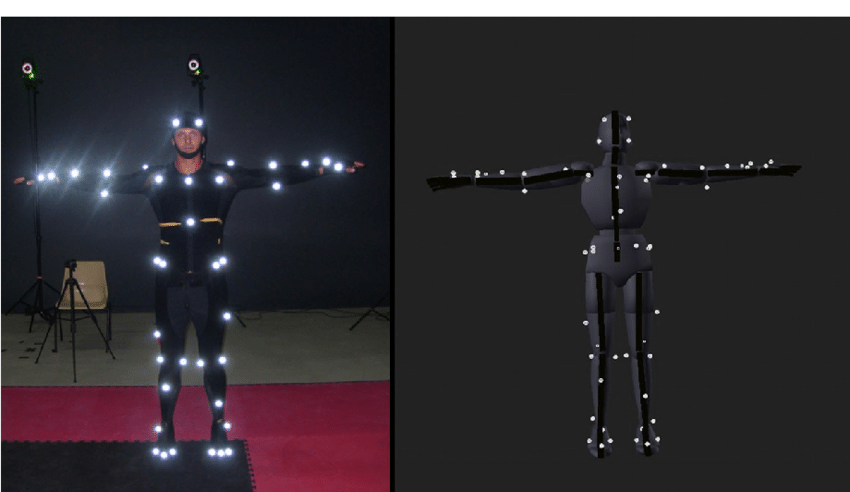
\includegraphics[width=0.6\textwidth]{figures/background/Optical.png}
	\caption{\href{https://www.researchgate.net/profile/Jacek-Hordyj/publication/283152771/figure/fig1/AS:669997391159296@1536751234023/Actor-wearing-suit-adjusted-for-optical-motion-capture-on-the-left-Virtual-model.png}
	{Optical Motion Capture suit}}
\end{figure}

Multiple high-speed cameras   \cite{Optical Motion Capture: Theory and Implementation,MOTION CAPTURE TO BUILD A FOUNDATION FOR A COMPUTER-CONTROLLED INSTRUMENT BY STUDY OF CLASSICAL GUITAR PERFORMANCE} or video cameras are used in optical motion capture systems to triangulate the position of each marker on the actor. This method involves using a series of synchronized cameras to capture markers placed in strategic locations on the body. More specifically, a number of synchronized cameras, an image acquisition system, a capturing area, and a special suit with markers are all required for the implementation of an optical motion capture system.The positions of the markers on the suit are designed to cover the necessary body parts.\\

Passive optical marker systems employ a variety of highly reflective markers of varying sizes that reflect light back to cameras. These markers can be velcroed to a body suit or applied directly to the skin. A ring of visible red, near red, or infrared strobe light emitting diodes (LEDs) around the camera lens generates the reflected light. The cameras' light sensitivity can be adjusted to reject other sources of light. Passive markers have the advantage of not requiring a power source such as batteries, wiring, or other electronic devices. The downside is that to the cameras, all of the markings appear to be the same. This means that if many markers are occluded and subsequently reappear in camera view, the cameras are unable to distinguish between them.\\

Active optical marker systems employ powered LEDs as markers.
Unlike passive markers, which reflect light back to cameras, these markers emit their own visible red or infrared light. These markers, like passive markers, can be adhered directly to the skin or velcroed to a body suit. The advantages of active markers are that each LED modulates and emits a unique frequency, resulting in each marker being uniquely identified. The disadvantage is that each LED must be powered, which necessitates the use of wires and related devices like batteries and circuit boards.
 
\pagebreak
\subsubsection{Non-Optical Motion Capture}
\subsubsection*{Inertial Motion Capture}
\begin{figure}[h]
	\centering
	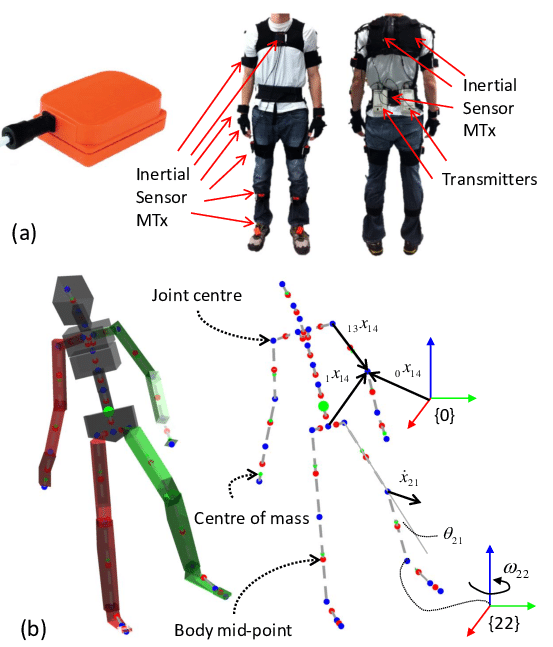
\includegraphics[width=0.4\textwidth]{figures/background/Inertial.png}
	\caption{\href{https://www.researchgate.net/profile/Matthew-Field-6/publication/257308000/figure/fig1/AS:613448983531582@1523269043700/a-The-inertial-sensor-MTx-left-14-and-positioning-of-the-sensors-and-wireless.png}
	{Inertial sensor suit}}
\end{figure}

Inertial sensors \cite{Kalman Filtering for Sensor Fusionin a Human Tracking System} rely on the property of bodies to maintain constant translational and rotational velocity unless perturbed by forces or torques. The vestibular system is a biological 3D inertial sensor located in the inner ear. It can detect both angular motion and linear acceleration of the head. The vestibular system is critical for maintaining eye balance and stabilization in relation to the environment. Advances in miniaturized and micro-machined sensor technologies, particularly silicon accelerometers and rate sensors, have made practical inertial tracking possible. A rate gyroscope measures angular velocity and provides the change in angle with respect to an initially known angle when integrated over time. Accelerations, including gravitational acceleration g, are measured by an accelerometer.\\

If the sensor's angle with respect to the vertical is known, the gravity component can be removed and velocity and position can be calculated using numerical integration. If no compensation is used, the noise and bias errors associated with small and inexpensive sensors make tracking orientation and position for long periods of time impractical. Drift and other errors can be reduced by combining signals from inertial sensors with those from aiding/complementary sensors and using knowledge about their signal characteristics.

\subsubsection*{Mechanical Motion Capture}

\begin{figure}[h]
	\centering
	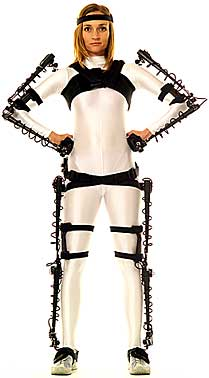
\includegraphics[width=0.3\textwidth]{figures/background/Mechanical.png}
	\captionsetup{labelformat=empty}
	\caption{\href{https://metamotion.com/images/gypsy4_standing.jpg}
	{Mechanical mocap suit}}
\end{figure}

Because of the external structure \cite{MOTION CAPTURE TO BUILD A FOUNDATION FOR A COMPUTER-CONTROLLED INSTRUMENT BY STUDY OF CLASSICAL GUITAR PERFORMANCE} that is attached to the performer, mechanical motion capture systems are also known as exoskeleton motion capture systems. These structures, which are typically made of rigid metal or plastic, have articulated joints with potentiometers that directly measure a performer's joint angles as he or she moves. One of the primary benefits of this direct measurement system is the absence of the need for cameras or other sensors. The system's main drawbacks are that the performer is restricted to the degrees of freedom of the structure and that the location of the sensor placement is fixed. If the performer attempts to move beyond the system's degrees of freedom, the structure may be damaged or broken.

\pagebreak

\subsubsection*{Magnetic Motion Capture}

\begin{figure}[h]
	\centering
	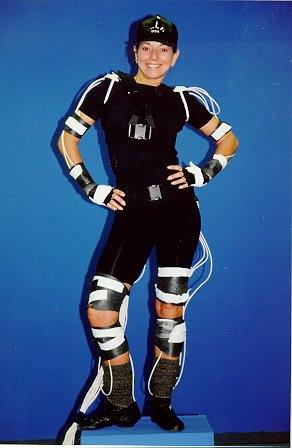
\includegraphics[width=0.3\textwidth]{figures/background/Magnetic.png}
	\captionsetup{labelformat=empty}
	\caption{\href{https://www.researchgate.net/profile/Jessica-Hodgins-2/publication/2359279/figure/fig4/AS:669524957331457@1536638597171/A-performer-wearing-a-motion-capture-apparatus-The-device-shown-is-a-full-body-magnetic.ppm}
	{Magnetic mocap suit}}
\end{figure}

Magnetic motion capture systems \cite{MOTION CAPTURE TO BUILD A FOUNDATION FOR A COMPUTER-CONTROLLED INSTRUMENT BY STUDY OF CLASSICAL GUITAR PERFORMANCE} work by measuring the low-frequency magnetic field produced by a source transmitter and relaying it to a receiver. Each transmitter and receiver have three orthogonal coils that measure magnetic flux between them and calculate the position and orientation of each sensor. One of the key advantages of these systems is that instead of the more conventional three degrees of position, each sensor transmitter/receiver pair may capture both orientation and position. However, sensors in the system, are susceptible to environmental metal, magnetic fields, and electrical sources such as rebar walls and floors, lights, cables, monitors, and computers. Shielding equipment and wiring requires special care. Despite their high accuracy, the sensors become nonlinear at the extremes of their range. 
\subsection{Neural Networks}
\subsubsection{Artificial Neural Network}
Machine Learning methods, particularly Artificial Neural Networks (ANNs), have shown promising capabilities in solving a wide range of complex problems. Neural networks are a class of machine learning techniques that attempts to recognize underlying relationships in a set of data using a process similar to how the human brain works. An artificial neural network (ANN) is a machine learning algorithm inspired by biological neural networks. The nodes in each ANN communicate with one another via connections. A deep network can represent functions of increasing complexity by adding more layers and units within a layer.

\pagebreak

 \begin{figure}[h]
	\centering
	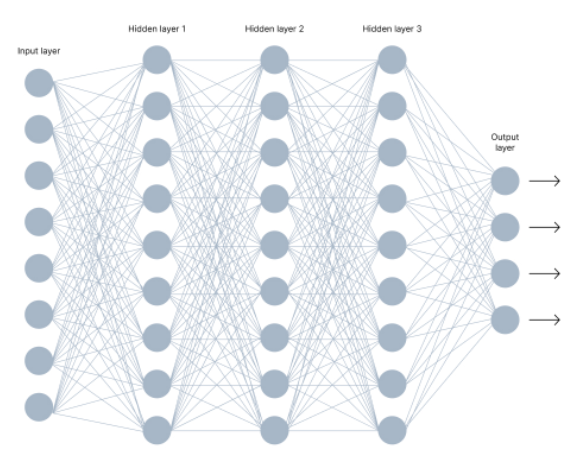
\includegraphics[width=0.6\textwidth]{figures/background/ANN.png}
	\captionsetup{labelformat=empty}
	\caption{\href{https://assets-global.website-files.com/5d7b77b063a9066d83e1209c/60d242974bcba9f8c670e03e_Group\%20806.jpg}
	{Neural Networks Architecture}}
\end{figure}

\subsubsection*{Artificial Neuron}
The fundamental building block of a neural network is a single neuron, which is also
 called a perceptron. More specifically, each neuron is a machine learning method that takes a set of features and their targets as input and tries to discover a line, plane, or hyperplane in two, three, or hyper-dimensional space that separates the classes. The sigmoid function is used to alter these characteristics.
 
 \begin{figure}[h]
	\centering
	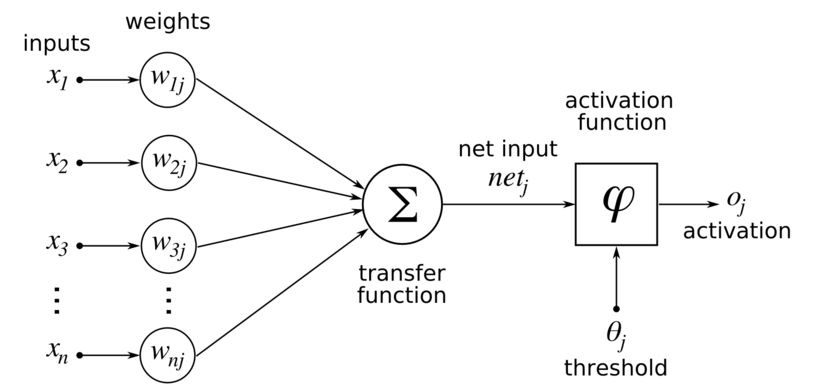
\includegraphics[width=0.6\textwidth]{figures/background/Neuron.png}
	\captionsetup{labelformat=empty}
	\caption{\href{https://commons.wikimedia.org/wiki/File:ArtificialNeuronModel_english.png}
	{Artificial Neuron}}
\end{figure}

Simple ANNs have an input layer and an output layer with zero to three hidden layers, whereas deep neural networks have no limit in the number of hidden layers. Multiple neurons make up a layer of a multilayer perceptron, and the input values as well as the bias values are assigned
during the training process.



\subsubsection*{Activation function}
The Activation function is used to determine whether or not the neuron will be activated. This means that it will use simpler mathematical operations to determine whether the neuron's input to the network is essential or not throughout the prediction phase. These mathematical functions are added to an artificial neural network to assist it in learning complex patterns in data. The reason that activation functions are essential parts of a ANN is that the combination of nonlinear activation functions from different neurons permits the network to approximate complex functions or distributions of data. Simpler, the most important feature of an activation function is to add non-linearity to a neural network. There are many activation functions, but here we show the most used functions.

 \begin{figure}[h]
	\centering
	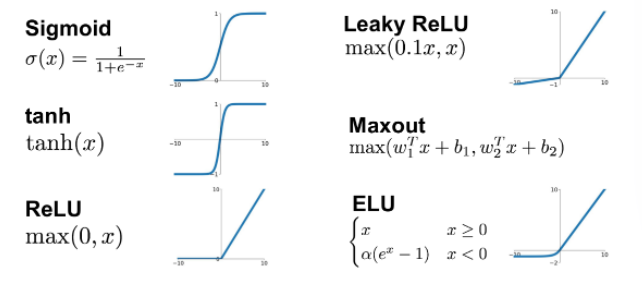
\includegraphics[width=0.6\textwidth]{figures/background/ActivationFunctions.png}
	\captionsetup{labelformat=empty}
	\caption{\href{https://datasciencepreparation.com/blog/articles/what-is-an-activation-function-what-are-commonly-used-activation-functions/}
	{Most common activation functions}}
\end{figure}

\subsubsection*{Loss Function}

One of the most important aspects of an ANN is the choice of the loss function \cite{The importance of the loss function in option valuation} . A loss function is incredibly simple at its core: It's a technique for determining how well your algorithm models your dataset. If the ANN predictions are completely incorrect, the loss function will return a higher value. Otherwise, it will return a lower value. However, minimizing the loss function doesn't necessarily mean that the prediction is getting closer to the desired results. There are some well-known categories of loss functions that may work on many simple ANN, but if the problem that the ANN has to solve is too complicated, it may need a custom loss function, that is special for the specific problem and ANN architecture. \\

In particular, the purpose of a loss function in an ANN is to adjust the weights and the bias during the training. If we could, we would find the perfect weights and bias for our ANN, but it has not yet been proven a formula that could do it. Therefore, these functions will try to find the adjustments, that are as close as to the perfect one's. \\

Pressingly, the loss function that is used is directly related to the activation function that is used in the neural network's output layer. Consider the output layer configuration to be a choice about the framing of the prediction problem, and the loss function selection to be the method for calculating the error for a given framing of the problem. The loss functions can be classified into two major categories depending upon the type of learning task we are dealing with Regression losses and Classification losses. In classification, we are trying to predict output from set of finite categorical values. Regression, on the other hand, deals with predicting a continuous value.

\subsubsection*{Back-propagation}

 \begin{figure}[h]
	\centering
	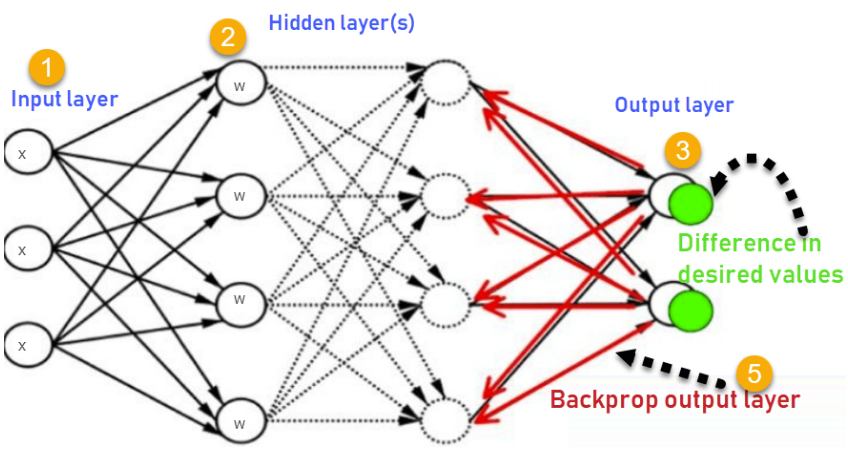
\includegraphics[width=0.8\textwidth]{figures/background/Backpropagation.png}
	\captionsetup{labelformat=empty}
	\caption{\href{https://www.guru99.com/images/1/030819_0937_BackPropaga1.png}
	{Backpropagation Algorithm}}
\end{figure}


The essence of neural net training is back-propagation. It is the practice of fine-tuning a neural net's weights based on the error rate obtained in the previous epoch. Proper weight tuning ensures lower error rates, increasing the model's reliability by increasing its generalization. \\

The back-propagation algorithm in neural networks computes the gradient of the loss function for a single weight using the chain rule. Unlike native direct computation, it efficiently computes one layer at a time. The back-propagation algorithm, allows the information from the cost to then flow backwards through the network, in order to compute the gradient. Back-propagation refers only to the method for computing the gradient, while another algorithm,
such as stochastic gradient descent, is used to perform learning using this gradient.

 
\subsubsection{Convolutional Neural Network}
Convolutional networks, \cite{Deep Learning} also known as convolutional neural networks or CNN, are a specialized kind of artificial neural network for processing data that has a known, grid-like topology. Examples include time-series data, which can be thought of as a 1D grid taking samples at regular time intervals, and image data, which can be thought of as a 2D grid of pixels. Convolutional networks are simply neural networks that use convolution in place of general matrix multiplication in at least one of their layers.\\

The main strengths of CNNs are to provide an efficient dense network which performs the prediction or identification etc. efficiently. CNNs are the most popular topic in the pool of deep learning, which is indeed very vast, and this is usually because of the ConvNets. Immense datasets are applied to CNNs, it is even considered that larger the data, greater the accuracy will result, otherwise other operations such as transfer learning shall be applied to expand the data. The power of CNN is to detect distinct features from images all by itself, without any actual human intervention.\\

There are multiple benefits of using this model as the state of art neural network. As it can be used in various fields and perform major tasks like facial recognition, analyzing documents, understanding climate, and image recognition and object identification etc. Deep learning has helped enormously in advancement of the science fields and CNN is the most popular one as it attains the benefits of providing maximum performance and efficiency.\\

Traditional neural network layers use matrix multiplication by a matrix of
parameters with a separate parameter describing the interaction between each input
unit and each output unit. This means every output unit interacts with every input
unit. Convolutional networks, however, typically have sparse interactions (also
referred to as sparse connectivity or sparse weights). This is accomplished by
making the kernel smaller than the input. For example, when processing an image,
the input image might have thousands or millions of pixels, but we can detect small,
meaningful features such as edges with kernels that occupy only tens or hundreds of
pixels. This means that we need to store fewer parameters, which both reduces the
memory requirements of the model and improves its statistical efficiency. It also
means that computing the output requires fewer operations. These improvements
in efficiency are usually quite large. If there are m inputs and n outputs, then
matrix multiplication requires m x n parameters and the algorithms used in practice
have O(m x n) run-time. If we limit the number of connections
each output may have to k, then the sparsely connected approach requires only
k x n parameters and O(k x n) run-time. For many practical applications, it is
possible to obtain good performance on the machine learning task while keeping
k several orders of magnitude smaller than m. \\


Each convolutional layer contains a series of filters known as convolutional kernels. The filter is a matrix of integers that are used on a subset of the input pixel values, the same size as the kernel. Each pixel is multiplied by the corresponding value in the kernel, then the result is summed up for a single value for simplicity representing a grid cell, like a pixel, in the output channel/feature map. In computer vision the input is often a 3 channel RGB image. For simplicity, if we take a grey-scale image that has one channel (a two dimensional matrix) and a 3x3 convolutional kernel (a two dimensional matrix). The kernel strides over the input matrix of numbers moving horizontally column by column, sliding/scanning over the first rows in the matrix containing the images pixel values. Then the kernel strides down vertically to subsequent rows. Note, the filter may stride over one or several pixels at a time, this is detailed further below.


 \begin{figure}[h]
	\centering
	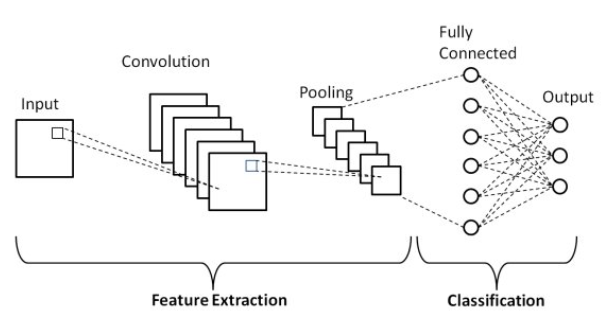
\includegraphics[width=0.8\textwidth]{figures/background/CNN.png}
	\captionsetup{labelformat=empty}
	\caption{\href{https://www.researchgate.net/publication/336805909/figure/fig1/AS:817888827023360@1572011300751/Schematic-diagram-of-a-basic-convolutional-neural-network-CNN-architecture-26.ppm}
	{Basic Convolution Neural Network Architecture}}
\end{figure}

\subsection{Related Work}
Recent work in the computer graphics and vision sectors have focused on developing digital tools for reconstructing, tracking, and evaluating human motion using visual input. More specifically, these digital tools that are easier and much cheaper to use, than mocap suits, and in the near future these methods have the potential to surpass the current technology that we talked about in the previous sections. At the moment, the resulting quality of these tools is not as good as the current technology, but many scientists propose state-of-the-art approaches in order to improve them.\\  

 \begin{figure}[h]
	\centering
	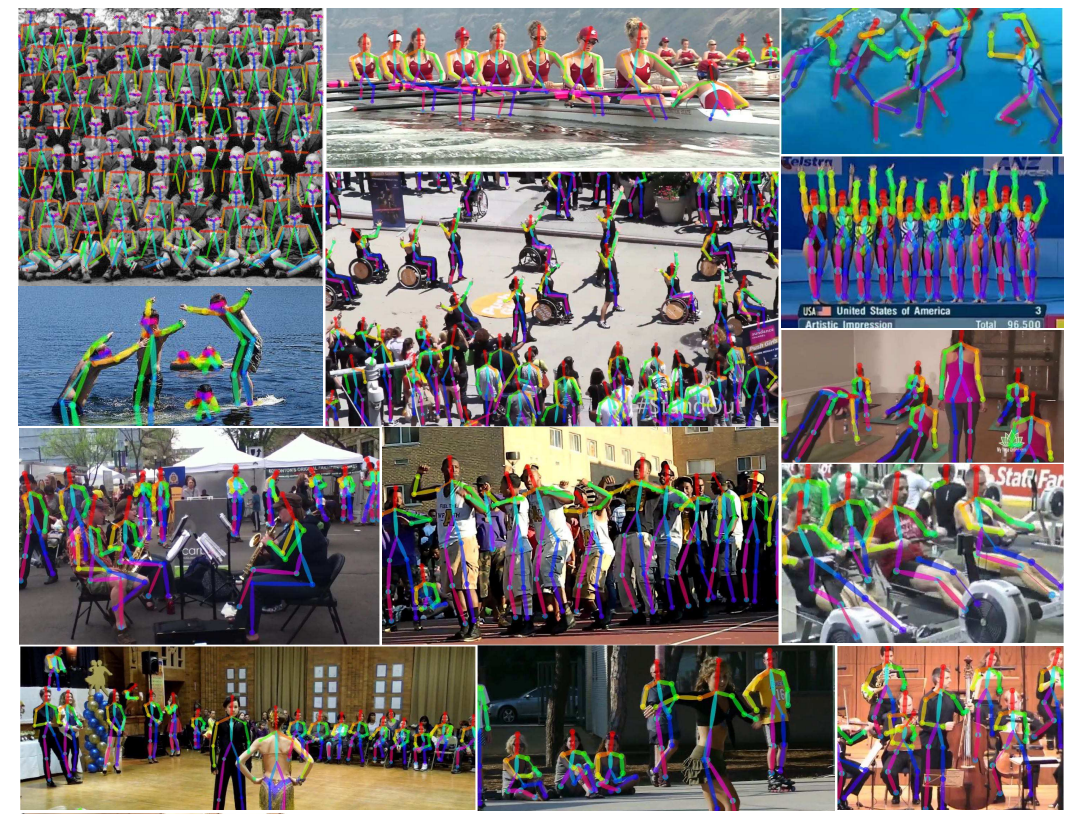
\includegraphics[width=0.6\textwidth]{figures/background/2D.png}
	\caption{\href{https://openaccess.thecvf.com/content_cvpr_2017/papers/Cao_Realtime_Multi-Person_2D_CVPR_2017_paper.pdf}
	{2D Multi-Person high accuracy human Pose estimation}}
\end{figure}

Reconstructing 3D human poses from real-world images in a variety of indoor and outdoor scenarios has a wide range of applications in entertainment, environmental awareness, and human-computer interaction. There are some ways to achieve that, but we will focus more on a specific procedure that estimates 3D human poses from a list of images or a video. Firstly, we will extract the 2D human poses from each image using some well-known Neural Networks specifically trained for this job. In particular, deep neural networks \cite{OpenPose,HrNet,AlphaPose} have revolutionized  2D pose estimation, producing accurate predictions even for poses with self-occlusions. These Neural Network can estimate the 2D human Pose in Real-Time with  high accuracy. These networks were trained with COCO dataset,  which contains over 200, 000 images and 250, 000 person instances labeled with 17 keypoints that are very easily recognisable. Even though the main difference in these network is the architecture and the training the 2D human Pose estimation, is very close. The main difference is the speed of the model and the hardware requirements of each model.\\

\pagebreak

 \begin{figure}[h]
	\centering
	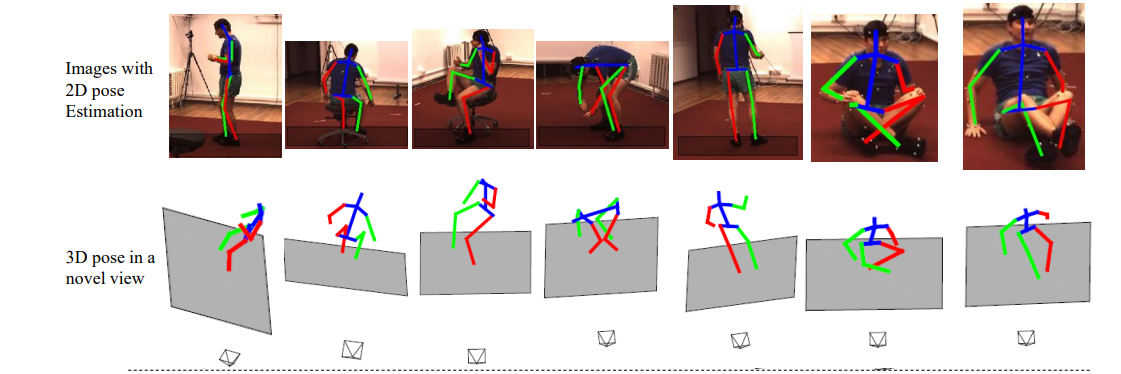
\includegraphics[width=1\textwidth]{figures/background/2D&3D.png}
	\caption{\href{https://arxiv.org/pdf/1612.06524.pdf}
	{2D and 3D human Pose difference in estimation}}
\end{figure}

In the last decade, the research community has paid close attention to inferring the 3D human pose from images or video. All the following studies \cite{Exploiting temporal information for 3D pose estimation,3D Human Pose Estimation from Deep Multi-View 2D Pose,3D Human Pose Estimation Using Convolutional Neural Networks with 2D Pose Information,3D Human Pose Estimation = 2D Pose Estimation + Matching}are proposing a deep neural network that can estimate 3D human poses  from a sequence of 2D human poses. Even though that each paper, proposes a different neural network architecture, all of them uses Human3.6M dataset and some of them, add to the training some other smaller datasets for further improvement of the results.\\

 \begin{figure}[h]
	\centering
	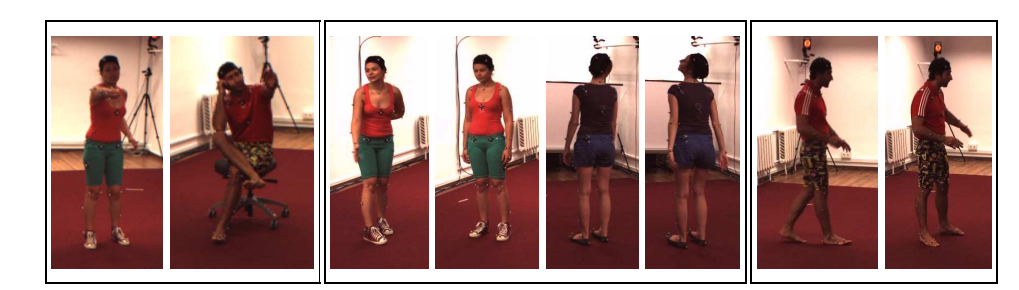
\includegraphics[width=1\textwidth]{figures/background/human36M.png}
	\caption{\href{https://vision.imar.ro/human3.6m/pami-h36m.pdf}
	{Examples of human poses in the Human3.6M dataset}}
\end{figure}

Recently, there has been some interest in systems whose components are trained using datasets of human motion capture . More specifically, a well-known and most used dataset is Human3.6M \cite{Human3.6M} which is a dataset of 3.6 million accurate 3D human poses collected by recording the performance of 5 female and 6 male subjects from four different perspectives in order to train realistic human sensing systems and evaluate the next generation of human pose estimation models and algorithms. \\



 
\subsection{Gait mocap clip Generation through a GAN}
All these methods try to estimate the 3D human Pose from a video. Another very interesting approach is to try to generate a BVH file that contains the mocap human pose information. The neural network that can achieve such task is a Generative adversarial network (GAN) \cite{ANIMGAN}. A GAN contains two neural networks the discriminator and the generator. Before the training starts, the former learns to separate fake data from real, and in the case of a fake, it includes how far it is from being real. The latter is creating some data, and its goal is to fool the discriminator by creating virtual data that looks real. Moreover in GAN's many researchers uses a type of layer, Long Short-Term Memory (LSTM) that are a type of recurrent neural network capable of learning order dependence in sequence prediction problems. Simply, this layer tries to find every association of the data, in our case, the association between the neighbours frames of the video. So, this paper, proposed a spatiotemporally-conditioned
GAN that generates a sequence that is similar to a given sequence in terms of semantics and spatiotemporal dynamics.Using LSTM-based generator and graph ConvNet discriminator, this system is trained end-to-end on a large gathered dataset of gestures, expressions, and actions.
\subsubsection{Dataset}
There are not many different walking datasets that can be used for this work. More specifically, Carnegie Mellon University which was created a huge motion capture dataset a decade ago that will be used in this Thesis. Moreover, It is possible for the skeleton that CMU proposed, to be rigged to a mixamo or another more modern skeleton through the blender and eventually import to game engines like Unity. This also means that we can increase the quantity of the CMU dataset by adding some mixamo or other well-known motion capture datasets (in BVH format) clips.\\

The CMU Graphics Lab Motion Capture Database (CMU) is by far the most extensive dataset of publicly available motion capture data. Many researchers within the community have used it to build prior models of human motion. This dataset was in Acclaim format. In particular, the Acclaim format is made up of two files, a skeleton file and a motion file. This was done knowing that a single skeleton works for many different motions most of the time and rather than storing the same skeleton in each of the motion files, it should be stored just once in another file. The skeleton file is the ASF file (Acclaim Skeleton File). The motion file is the AMC file (Acclaim Motion Capture data). In addition, some people created python software that converts the Acclaim files into BVH files. It means that these files can be imported into the blender for further usage.\\

There some other datasets like mixamo, that contains high-quality motion capture but it is not always free. The primary purpose of these motion capture is game construction of video clip animation. In this thesis, it is important to obtain a significant amount of motion capture, something that only CMU can offer for free. Fortunately, we can still modify the mixamo dataset (rig the mixamo skeleton to CMU skeleton) and merge it to the CMU dataset.\\

This dataset will train a neural network to classify for the training when the skeleton model
of the dataset is walking. Some approaches train a neural network with the CMU mocap
clips as the dataset. The CMU skeleton has 31 joints, and each joint is described by the
position (XYZ) and the rotation (XYZ), a total of 6 variables. That sum up to 186 variables
for each frame. Each clip has 3198 frames, and we use 1073 clips from the dataset. So the
dataset final form is a array with  these dimensions (1073,3198,186).\\

In addition to these clips, we added some noise z using a normal or uniform distribution to some of the clips in order to classify some of them as fake. This was necessary for the network, in order to understand, during the training what a  false sample looks like. So, the now has a form of (1500,3198,186), which means that we were added 427 false samples. \\

However, it is still a small dataset. There a machine learning strategy, that allows you to increase your dataset, it is called data augmentation. More specifically, data augmentation is a strategy that enables practitioners to significantly increase the diversity of data available for training models, without actually collecting new data. The data augmentation in our case includes random rotation ([-$45^o$, $45^o$]) and random scale ([0.5, 1.5]). So the final form of the dataset was (10000,3198,186).
\subsubsection{Generative Adversarial Networks}
There are not many different walking datasets that can be used for this work. More specifically, Carnegie Mellon University which was created a huge motion capture dataset a decade ago that will be used in this Thesis. Moreover, It is possible for the skeleton that CMU proposed, to be rigged to a mixamo or another more modern skeleton through the blender and eventually import to game engines like Unity. This also means that we can increase the quantity of the CMU dataset by adding some mixamo or other well-known motion capture datasets (in BVH format) clips.\\

The CMU Graphics Lab Motion Capture Database (CMU) is by far the most extensive dataset of publicly available motion capture data. Many researchers within the community have used it to build prior models of human motion. This dataset was in Acclaim format. In particular, the Acclaim format is made up of two files, a skeleton file and a motion file. This was done knowing that a single skeleton works for many different motions most of the time and rather than storing the same skeleton in each of the motion files, it should be stored just once in another file. The skeleton file is the ASF file (Acclaim Skeleton File). The motion file is the AMC file (Acclaim Motion Capture data). In addition, some people created python software that converts the Acclaim files into BVH files. It means that these files can be imported into the blender for further usage.\\

There some other datasets like mixamo, that contains high-quality motion capture but it is not always free. The primary purpose of these motion capture is game construction of video clip animation. In this thesis, it is important to obtain a significant amount of motion capture, something that only CMU can offer for free. Fortunately, we can still modify the mixamo dataset (rig the mixamo skeleton to CMU skeleton) and merge it to the CMU dataset.\\

This dataset will train a neural network to classify for the training when the skeleton model
of the dataset is walking. Some approaches train a neural network with the CMU mocap
clips as the dataset. The CMU skeleton has 31 joints, and each joint is described by the
position (XYZ) and the rotation (XYZ), a total of 6 variables. That sum up to 186 variables
for each frame. Each clip has 3198 frames, and we use 1073 clips from the dataset. So the
dataset final form is a array with  these dimensions (1073,3198,186).\\

In addition to these clips, we added some noise z using a normal or uniform distribution to some of the clips in order to classify some of them as fake. This was necessary for the network, in order to understand, during the training what a  false sample looks like. So, the now has a form of (1500,3198,186), which means that we were added 427 false samples. \\

However, it is still a small dataset. There a machine learning strategy, that allows you to increase your dataset, it is called data augmentation. More specifically, data augmentation is a strategy that enables practitioners to significantly increase the diversity of data available for training models, without actually collecting new data. The data augmentation in our case includes random rotation ([-$45^o$, $45^o$]) and random scale ([0.5, 1.5]). So the final form of the dataset was (10000,3198,186).
\subsubsection{Evaluation of the approach}
Unfortunately, the results of this approach were terrible. The main reason was the small dataset that we were able to find for free. Even though we tried to do data augmentation in our dataset, there is a limitation. The main limitation of data augmentation arises from the data bias, i.e. the augmented data distribution can be quite different from the original one. This data bias leads to a sub-optimal performance of existing data augmentation methods. In particular, the generator could not improve his results, so the output was something a little better than the  noise z using a normal or uniform distribution that we sampled in the generator in the initial phase and the humanoid was doing independent random moves in each frame of the motion. The dataset limitation in this area is something that many researchers have noticed, and the goal was to try to increase the dataset even with poorer quality with this model. 
\newpage
\section{Requirements}
\subsection{Hardware}
As we mentioned in previous sections, models that estimate human pose, particularly models that estimate 2D poses from a single image, require above-average hardware. These models can be loaded on the CPU but the speed that the model needs to run the estimation is about 0.2-0.3 frames per second in Intel Core i7-7700HQ (2.8GHz) which is considered an above-average CPU. On the other hand, having a GPU with at least 2 GB VRAM (that is the minimum allocated space that the models need to be loaded), the speed that the model needs to run the estimation is about 4-5 frames per second in NIVIDIA GeForce GTX 1050 which also is considered an above-average GPU. The difference in speed is enormous, GPU is about 20 times faster than the CPU. The application was tested on a laptop, MSI GL72M 7RDX. During the run-time, the hardware of the laptop is shown in the figure from the application MSI DRAGON CENTER:

\begin{figure}[h]
	\centering
	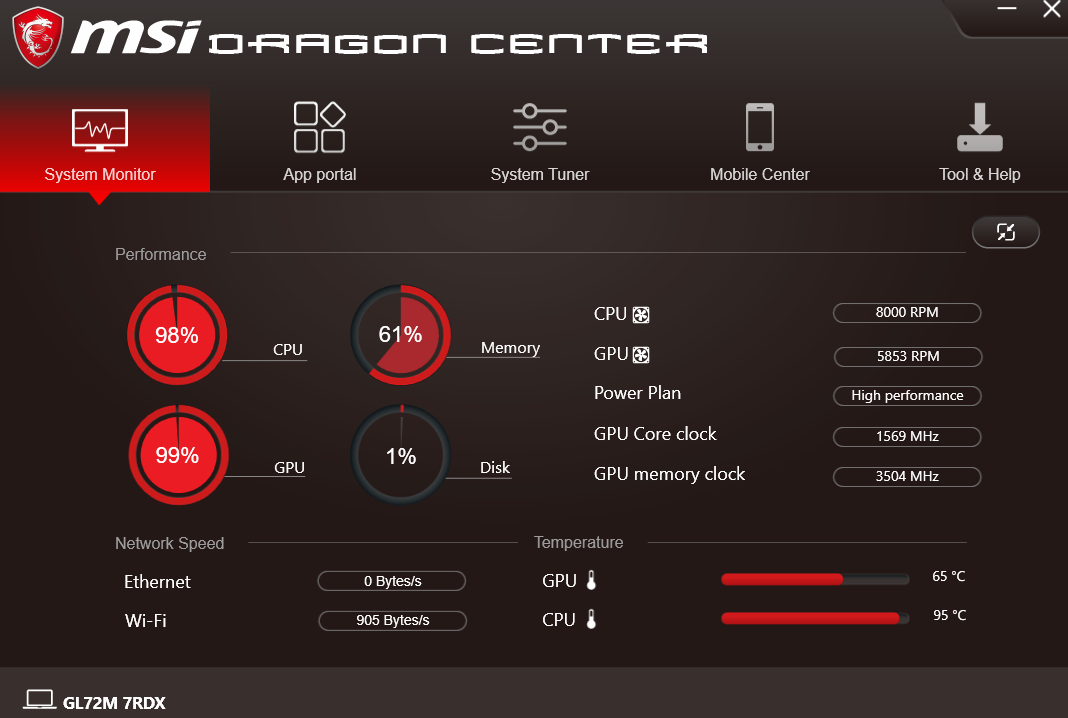
\includegraphics[width=0.9\textwidth]{figures/Requirements/Perfomance.png}
	\captionsetup{labelformat=empty}
	\caption{ MSI GL72M 7RDX performance stats}
\end{figure}
\subsection{Input requirements}
The input of the algorithm is a video. We suggest that the resolution of the video is at least 720p, in order that every human joint can be easily recognizable by the model. The best video resolution for the specific version of the application is 1080p, which maximizes the algorithm speed as well as the resulting quality. However, the results (depends on the movement complexity) may not be clear enough to be imported directly to a game engine studio so this application is addressed to animators. Nevertheless, mocap clips always needed to be cleared (discard some frames and keep the best for the motion), so it was something to be expected. Moreover, there are some rules that if the video-creator follow, he will improve the quality of the model estimation. Firstly, the camera should be motionless, because it affects the position estimation. Secondly, the person's joints should be visible, otherwise, the model may struggle to specify left from right joints, (legs and arms). Another tip is that whole body of the person should be visible for every frame of the video, and the distance between him and the camera should be greater than two meters and less than six meters. The most important idea that would help improve the estimation quality would be if the user could upload a slow-motion video, that will contain the motion of the video in great detail since all the sharp movement will now become smoother, more detailed, and slower between each frame movements.
\pagebreak
\subsection{Application's Workflow}
The Application's workflow can be divided into three parts. The first part is quite simple, the user imports the video of his preference into the Application chooses the folder that he wants to save the results, and presses submit as it is shown in the figures above. 

\pagebreak

\begin{figure}[htp]
	\centering
	{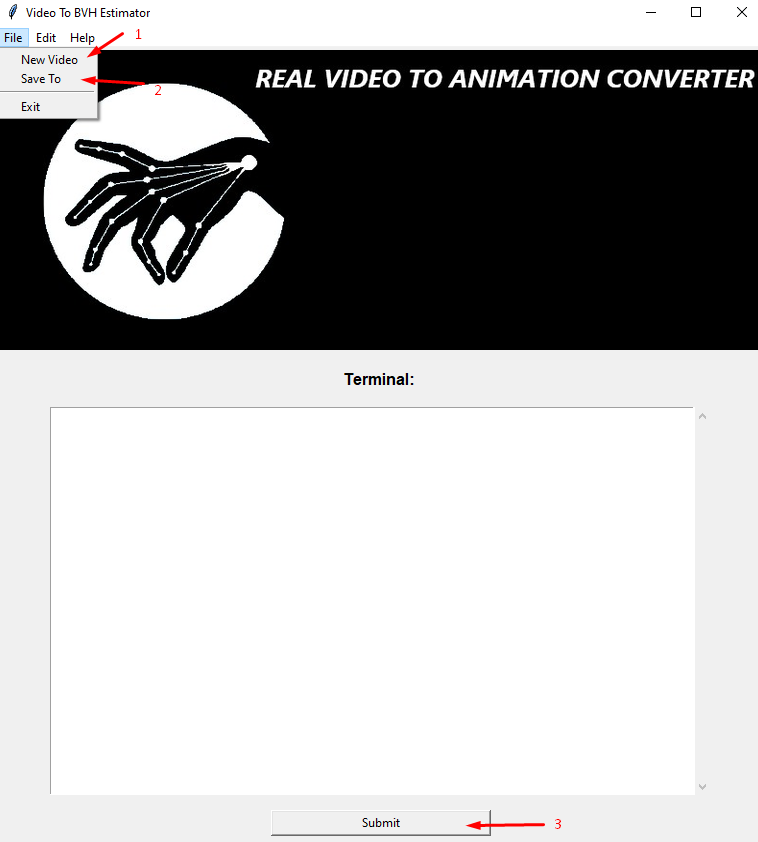
\includegraphics[height=9cm,width=0.48\linewidth]{figures/Requirements/Workflow1_1.png}}
	\hspace{1em}%
	{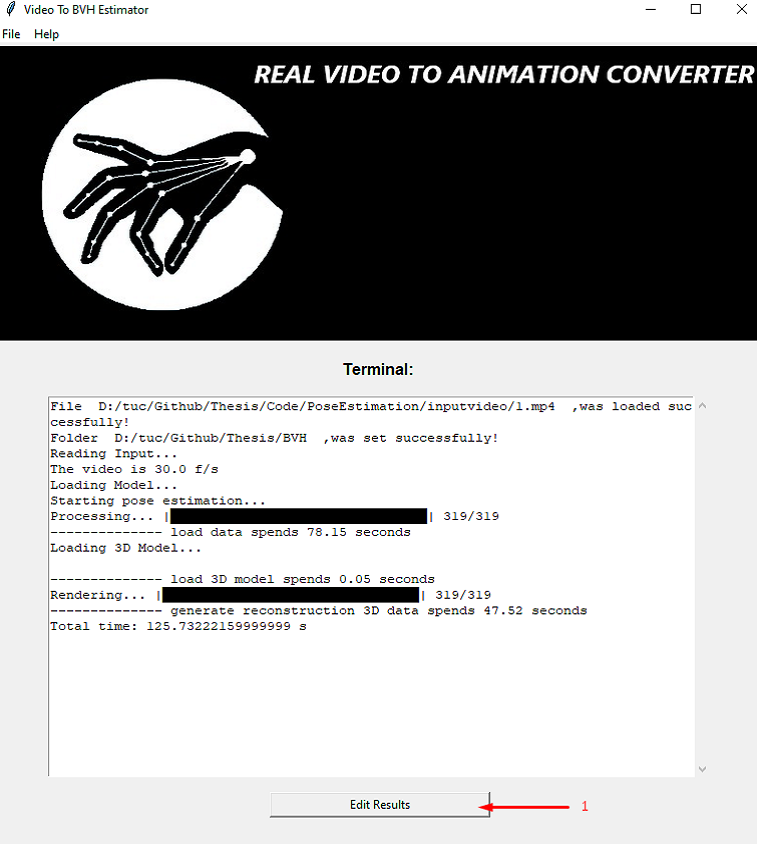
\includegraphics[height=9cm, width=0.48\linewidth]{figures/Requirements/Workflow1_2.png}}
	\captionsetup{labelformat=empty}
	\caption{Input Phase}
\end{figure}

In the above figure, in the left image, we show how to give new input to the Application. In the right image, we show the results that the user should see after a successful video to animation conversion as well as the way to go to the next panel.\\\\


 \begin{figure}[h]
	\centering
	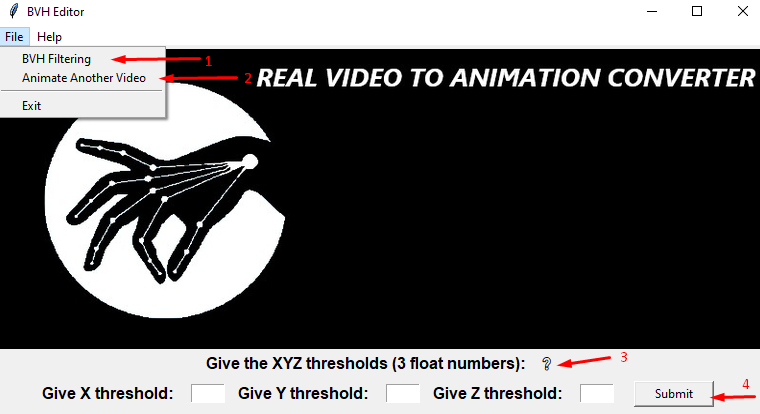
\includegraphics[width=0.55\textwidth]{figures/Requirements/Workflow2_1.png}
	\captionsetup{labelformat=empty}
	\caption{Editing Phase}
\end{figure}

\pagebreak

In the above figure, in the top image, the user can multiply with a number of his preference for each dimension in $R^3$. By doing so, he can increase or decrease the position speed. In the right image, the user can press the left button to filter the BVH motion data in order to reduce the noise, or can press the right button in order to return to the first panel and animate more videos. In addition, if the user does not understand something from the application, he can hover the mouse over the question marks to display some tips.\\\\


\begin{figure}[htp]
	\centering
	{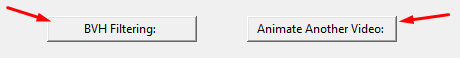
\includegraphics[height=10cm,width=0.48\linewidth]{figures/Requirements/Workflow2_2.png}}
	\hspace{1em}%
	{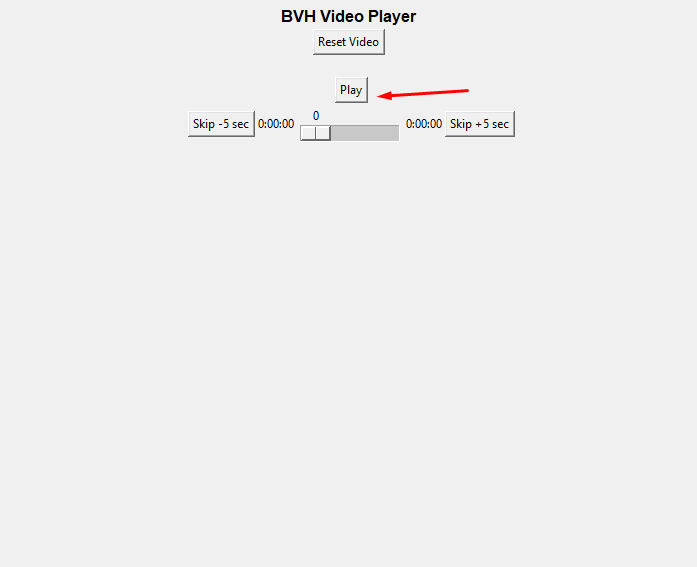
\includegraphics[height=10cm, width=0.48\linewidth]{figures/Requirements/Workflow2_3.png}}
	\captionsetup{labelformat=empty}
	\caption{BVH Video Player}
\end{figure}

The animators may change several things during this phase, so it would be very helpful if they could actually see the motion displayed in this panel. Therefore, if the pressed play, an mp4 of the motion starts playing. If the user changes something in the motion, either they filter the BVH or edit the position of the skeleton, in order to reload the mp4, they need to press reset the video. Unfortunately, this procedure is time-consuming, depending form the CPU the user has the speed of conversion from a BVH to an mp4, is about 10 frames per second.

\pagebreak

\begin{figure}[htp]
	\centering
	{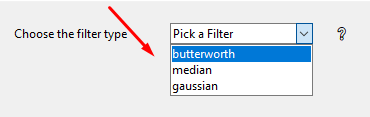
\includegraphics[height=3cm,width=0.48\linewidth]{figures/Requirements/Workflow3_1.png}}
	\hspace{1em}%
	{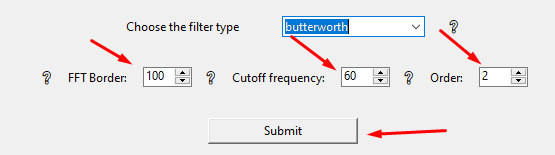
\includegraphics[height=3cm, width=0.48\linewidth]{figures/Requirements/Workflow3_2.png}}
	\captionsetup{labelformat=empty}
	\caption{Filtering Phase}
\end{figure}

In this phase the user can choose a filter of his preference, and insert the parameters that each filter need in order to work. The filter feature is added due to the fact that the estimation that the neural networks do, contain some noise, and these filters can significantly reduce it, or in some cases almost vanished it, which saves a lot of time from the animators.
\newpage
\section{Implementation}
\subsection{Mocap Dataset Augmentation using pretrained models}
\subsubsection{Dataset Augmentation}
\subsubsection{Available Pretrained Models}
\subsubsection{Alpha-pose model}
\subsubsection{Orientation and location estimation}
\subsection{Animator Tools}
\subsubsection{Biovision Hierarchical (BVH)}
\subsubsection{Fast BVH Editing}
\subsubsection{BVH Filtering}
\subsection{Windows Application}
\subsubsection{Application's UI}
\subsubsection{Tkinter library}
\subsubsection{Construction of the Application }
\newpage
\section{Evaluation}
\subsection{Algorithm Accuracy}
\subsection{Comparing Result}
\newpage
\section{Discussion}
\subsection{Drawbacks of our Work}
\subsection{Future Approaches}
\newpage
\begin{thebibliography}{9}

\bibitem{Efficient Content-Based Retrieval of Motion Capture Data}
M{\"u}ller, Meinard and R{\"o}der, Tido and Clausen, Michael ACM SIGGRAPH 2005 Papers 677--685\\

\bibitem{Exploiting temporal information for 3D pose estimation}
Rayat Imtiaz Hossain, Mir, and James J. Little. "Exploiting temporal information for 3D pose estimation." arXiv e-prints (2017): arXiv-1711.\\

\bibitem{3D Human Pose Estimation from Deep Multi-View 2D Pose}
Schwarcz, Steven, and Thomas Pollard. "3d human pose estimation from deep multi-view 2d pose." 2018 24th International Conference on Pattern Recognition (ICPR). IEEE, 2018.\\

\bibitem{3D Human Pose Estimation Using Convolutional Neural Networks with 2D Pose Information}
Park, Sungheon, Jihye Hwang, and Nojun Kwak. "3d human pose estimation using convolutional neural networks with 2d pose information." European Conference on Computer Vision. Springer, Cham, 2016.\\

\bibitem{Review on Motion Capture Technology}
Rahul, M. "Review on motion capture technology." Global Journal of Computer Science and Technology (2018).\\

\bibitem{Optical Motion Capture: Theory and Implementation}
Guerra-Filho, Gutemberg. "Optical Motion Capture: Theory and Implementation." RITA 12.2 (2005): 61-90.\\

\bibitem{Kalman Filtering for Sensor Fusionin a Human Tracking System}
Corrales Ramón, Juan Antonio, Francisco A. Candelas-Herías, and Fernando Torres. Kalman filtering for sensor fusion in a human tracking system. Intech, 2010.\\

\bibitem{MOTION CAPTURE TO BUILD A FOUNDATION FOR A COMPUTER-CONTROLLED INSTRUMENT BY STUDY OF CLASSICAL GUITAR PERFORMANCE}
 Norton, Jonathan Carey. Motion capture to build a foundation for a computer-controlled instrument by study of classical guitar performance. Stanford University, 2008.\\
 
\bibitem{Deep Learning}
https://www.deeplearningbook.org/\\

\bibitem{ANIMGAN: A SPATIOTEMPORALLY-CONDITIONED GENERATIVE ADVERSARIAL NETWORK FOR CHARACTER ANIMATION}
Mirzaei, Maryam Sadat, et al. "Animgan: A spatiotemporally-conditioned generative adversarial network for character animation." 2020 IEEE International Conference on Image Processing (ICIP). IEEE, 2020.\\

\bibitem{3D Human Pose Estimation = 2D Pose Estimation + Matching}
Chen, Ching-Hang, and Deva Ramanan. "3d human pose estimation= 2d pose estimation+ matching." Proceedings of the IEEE Conference on Computer Vision and Pattern Recognition. 2017.\\

\bibitem{The importance of the loss function in option valuation}
Christoffersen, Peter, and Kris Jacobs. "The importance of the loss function in option valuation." Journal of Financial Economics 72.2 (2004): 291-318.\\

\bibitem{Human3.6M}
Ionescu, Catalin, et al. "Human3. 6m: Large scale datasets and predictive methods for 3d human sensing in natural environments." IEEE transactions on pattern analysis and machine intelligence 36.7 (2013): 1325-1339.\\

\bibitem{OpenPose}
Cao, Zhe, et al. "Realtime multi-person 2d pose estimation using part affinity fields." Proceedings of the IEEE conference on computer vision and pattern recognition. 2017.\\

\bibitem{HrNet}
Sun, Ke, et al. "Deep high-resolution representation learning for human pose estimation." Proceedings of the IEEE/CVF Conference on Computer Vision and Pattern Recognition. 2019.\\

\bibitem{AlphaPose}
Fang, Hao-Shu, et al. "Rmpe: Regional multi-person pose estimation." Proceedings of the IEEE international conference on computer vision. 2017.\\

\bibitem{ANIMGAN}
Mirzaei, Maryam Sadat, et al. "Animgan: A spatiotemporally-conditioned generative adversarial network for character animation." 2020 IEEE International Conference on Image Processing (ICIP). IEEE, 2020.\\

\bibitem{Human Action Generation with Generative
Adversarial Networks}
Kiasari, Mohammad Ahangar, Dennis Singh Moirangthem, and Minho Lee. "Human action generation with generative adversarial networks." arXiv preprint arXiv:1805.10416 (2018).\\

\bibitem{SPPE}
Zhang, Feng, Xiatian Zhu, and Chen Wang. "Single Person Pose Estimation: A Survey." arXiv preprint arXiv:2109.10056 (2021).\\

\bibitem{YOLO-Pose}
Maji, Debapriya, et al. "YOLO-Pose: Enhancing YOLO for Multi Person Pose Estimation Using Object Keypoint Similarity Loss." arXiv preprint arXiv:2204.06806 (2022).\\

\bibitem{YOLOv3}
Redmon J, Farhadi A, "YOLOv3: an Incremental Improvement," https://arxiv.org/
abs/1804.02767, 2018.

\bibitem{HourGlass}
Newell, Alejandro, Kaiyu Yang, and Jia Deng. "Stacked hourglass networks for human pose estimation." European conference on computer vision. Springer, Cham, 2016.

\bibitem{Attention Mechanism Exploits Temporal Contexts: Real-time 3D Human Pose Reconstruction}
Liu, Ruixu, et al. "Attention mechanism exploits temporal contexts: Real-time 3d human pose reconstruction." Proceedings of the IEEE/CVF Conference on Computer Vision and Pattern Recognition. 2020.\\

\bibitem{3D human pose estimation in video with temporal convolutions and semi-supervised training}
Pavllo, Dario, et al. "3d human pose estimation in video with temporal convolutions and semi-supervised training." Proceedings of the IEEE/CVF Conference on Computer Vision and Pattern Recognition. 2019.\\

\bibitem{Mean Filtering}
Chandrinos, Aristeidis. "The Challenge of Predicting OAG Progression from the Initial Visual Field Test." Signal 4: 6.\\

\bibitem{Gaussian Filtering}
Ramamurthy, Arjun. "An All Digital Implementation of Constant Envelope: Bandwidth Efficient GMSK Modem using Advanced Digital Signal Processing Techniques." Wireless personal communications 52.1 (2010): 133-146.\\

\bibitem{Butterworth Filtering}
Cuadrado, Javier, Florian Michaud, Urbano Lugrís, and Manuel Pérez Soto. "Using accelerometer data to tune the parameters of an extended kalman filter for optical motion capture: Preliminary application to gait analysis." Sensors 21, no. 2 (2021): 427.\\

\bibitem{Tkinter 1}
Lundh, Fredrik. "An introduction to tkinter." URL: www. pythonware. com/library/tkinter/introduction/index. htm (1999).\\

\bibitem{Tkinter 2}
Grayson, John E. Python and Tkinter programming. Manning Publications Co. Greenwich, 2000.\\

\bibitem{MS COCO}
Lin, Tsung-Yi, Michael Maire, Serge Belongie, James Hays, Pietro Perona, Deva Ramanan, Piotr Dollár, and C. Lawrence Zitnick. "Microsoft coco: Common objects in context." In European conference on computer vision, pp. 740-755. Springer, Cham, 2014.\\

\bibitem{AP}
https://jonathan-hui.medium.com/map-mean-average-precision-for-object-detection-45c121a31173\\

\bibitem{OCHuman}
Zhang, Song-Hai, Ruilong Li, Xin Dong, Paul Rosin, Zixi Cai, Xi Han, Dingcheng Yang, Haozhi Huang, and Shi-Min Hu. "Pose2seg: Detection free human instance segmentation." In Proceedings of the IEEE/CVF Conference on Computer Vision and Pattern Recognition, pp. 889-898. 2019.\\

\end{thebibliography}

 
% \section{Introduction} \label{ch1}
% \input{sources/1_introduction.tex} 

\label{EndOfText}

\label{endOfDoc}

\end{document}
